\documentclass[sigconf]{acmart}

\usepackage{graphicx}
\usepackage{hyperref}
\usepackage{todonotes}

\usepackage{endfloat}
\renewcommand{\efloatseparator}{\mbox{}} % no new page between figures

\usepackage{booktabs} % For formal tables

\settopmatter{printacmref=false} % Removes citation information below abstract
\renewcommand\footnotetextcopyrightpermission[1]{} % removes footnote with conference information in first column
\pagestyle{plain} % removes running headers

\newcommand{\TODO}[1]{\todo[inline]{#1}}

\begin{document}
\title{Big Data Applications for Visualizations}


\author{Jacob Tibenkana}
\orcid{1234-5678-9012}
\affiliation{%
  \institution{Indiana University}
  \streetaddress{107 S. Indiana Avenue}
  \city{Bloomington}
  \state{Indiana}
  \postcode{47405-7000}
}
\email{jtibenka@iu.edu}

% The default list of authors is too long for headers}
\renewcommand{\shortauthors}{J. Tibenkana}


\begin{abstract}
We live in the age of information. Data is everywhere and is increasingly becoming a major player in the way people and companies make decisions. There are many data analytics companies today to help other companies make decisions based on the data they collect. People consult Yelp for decision making on a restaurant, barber shops, banks to use, etc. More however, the machinery we have today from the industrial age is programmed using data we have collected over the years. There is a challenge though, we cannot take random information and find an application for it without first cleaning it and presenting it in a friendlier human way, so people can make sense of it and determine its applications. Hence, enter the field of Data Visualizations. 
\end{abstract}

\keywords{i523}

\maketitle

%here begins the body of the document
\section{Introduction}
During the industrial age, machinery was the element that drove production, it stimulated economies, and ushered in a new era where people moved away from hand held tool. (history). According to the History website:
Industrialization marked a shift to powered, special-purpose machinery, factories and mass production. The iron and textile industries, along with the development of the steam engine, played central roles in the Industrial Revolution, which also saw improved systems of transportation, communication and banking. (History)
Today, the discoveries and creations that came from the industrial revolution still influence our societies from automobile production, food production, manufacturing jobs, weapons creations, etc., but something else special is also influencing our world now. This is the information age. It can be argued that the human species have been collecting information since they became conscious of themselves and their environment. This has occurred in the past thousand years. Given that it now 2017, this can equate to a massive amount of data. If one must find a solution using information we know, it may be simple if it’s from a single scenario, but what about data collected for years or from multiple sources. This can result in too much information to be analyzed and tracked by the human brain, which will eventually become overwhelming. So how do we get around this? Luckily, due to the advances made in the informational age with computing in big data, programming languages have been made to take a collective of information in files such as CSV and XML or the traditional excel files of information to present it in a more human friendly way.
People usually use Microsoft Excel to plot graphs and charts of information to show trends, values, etc., and we still use excel to do it today. However, we have more options to dive deeper into big data and link different programs to produce reports. Some of these ways include but not limited to, Google Chart, Tableau, D3, Fusion chart, High charts, Canvas, Qlikview, Datawrapper, Microsoft Power BI, and Oracle Visual Analyzer. (PromptCloud) The softwares listed above are all good to use for data visualization and analysis. Some of them like Tableau do not require any coding knowledge. Even with this long list of programs to use, there is still more. One can use programming languages such as R, Python, Java, etc. to provide a statistical approach to data and compute algorithms that provide solutions from the information we see and collect in the world. This will later be shown where R with Latex can analyze data from the Titanic. However, before we get to that, we should explore data regarding to visualizations and the options we have in the information age. 

\section{Data visualization}
What is Data visualization and why is it Important? According to the SAS website:
Data visualization is the presentation of data in a pictorial or graphical format. It enables decision makers to see analytics presented visually, so they can grasp difficult concepts or identify new patterns. With interactive visualization, you can take the concept a step further by using technology to drill down into charts and graphs for more detail, interactively changing what data you see and how it’s processed. (SAS)
in other words, data visualization is taking data or pieces of information and providing it in images, charts, and graphs so people can see the whole picture. Look at how different pieces work and impact to make a puzzle, which can help decision makers to proceed. The SAS website goes on to say, the idea of using images to conceive data has been in use for hundreds of years, from maps and graphs used in the 1600s to the pie chart that showed up in the 19th century. Today however, data visualization has become its own field of science and art that will impact the corporate landscape. (SAS) Furthermore, the way humans look at information, using pictures to visualize large amount information can be easier than staring at large spreadsheets or reports of text or numbers. Can you imagine what it would be like staring at your cell phone home screen and each app was in the form words or numbers (0s and 1s), it would not be pleasant and that’s why we have icon images to help visualize the apps. Having image icons for apps in our cell phones helps identify really quickly what the apps are and if there is red 1 or red 2 hovering over the image, this notifies us that there is something new that has happened and we should look into it. However, this goes further than just what is on our cell phones, the SAS website says, retail bankers use big data visualizations to improve their customer service and relations.  Retail banking is not the only entity that uses this. Many of us have filled out customer surveys at our favorite corporate chain. (SAS) One can imagine that this information is analyzed visually to see how the company is doing and look at where improvements can be made. At the end of the day, if a company is meeting their customer’s needs, the customer will typically coming back for more business and they will refer their family and friends to this company, which drives up sales and the up most excellence in delivery and revenue.
According to Rosemary Radich in her article Big Data For Humans: The Importance of Data Visualization, companies look at the data itself and for an individual who can analyze that data, because the data available today to businesses and costumers can be crushing. The human brain can only process a couple of items at a time. Therefore, the need for people who can accurately present and communicate the data effectively is critical. “Everyone has heard the old moniker garbage in – garbage out. It is a simple way of saying that machine learning is only as good as the data, algorithms, and human experience that goes into them. But even the best results can be thought of as garbage if no one can see and understand the value of the output (Radich, May 8, 2017) Radich makes a good point here; It is important that people can understand the result. Otherwise all the work spent to make a report can be wasteful if no one understands its purpose. 
What programs do people and companies use to make the “garbage” (Radich, May 8, 2017) presentable in a purposeful way? It was mentioned above that programs like Google Chart, Tableau, etc. can be used to make visualizations for audiences to gain further insight of what the data is showing. Let’s explore a few of these programs such as Google Chart and Tableau. 

\section{Google Chart and Tableau}
According to the Google developer website, Google Chart allows users to use various chart types to present or plot their data. With Google Chart one can configure extensive sets of data to perfectly match their website. It can visualize data on old internet explorers and can be carried over to IOS and Android with no plugins needed. It also allows people to connect to their information in real time by a various data linking tools and conventions. (Google Developers website) Finances Online says, “Google Charts offers users with an online tool that enables users to display their data on their website via simple or attractive visualizations.” (FinancesOnline) It is also free. Using google Chart people can make Geo Charts, Histograms, Area Charts, Org Charts, Timelines, Scatter Plots, Bar Chats, Stepped Area Charts, Bubble Charts, Tree maps, Gauges, Colum Charts, Combo Charts, Line Charts, Donut Charts, Tables, and Candlestick Charts. (Google Developers website) Clearly, there are many options one has with Google chart depending on what visuals they want to create. Simply put, use google spread sheets to store information and then use Google Chart to display this information in the options of visuals listed above. This can also be done through another program called Tableau. 

According to the Tableau website, Tableau is a program that allows to connect and visualize one’s information in mintues; it is 10 to 100 times faster than other visual programs. It does not require programming knowledge and almost anyone can use it. It allows you to explore any data, updates automatically, and takes seconds to share visualizations on the web and mobile devices. “Wells Fargo wrangles data from over 70 million customers to redesign customer banking portals” through Tableau. (Tableau) This clearly falls in the realm of big data visualization. Finances Online says, “Tableau provides beautiful data analytics that can help all business make better business decisions.” (FinancesOnline) Tableau offers more visual options than google chart that are used in the Healthcare analytics, Education analytics, Government analytics, IT analytics, Marketing analytics, Big Data, Maps, Amazon Web services, and Google itself. (Tableau) Below in Figure 1, Idatalabs compares the use of Google Chart vs Tableau, and other competitors for business intelligence. 

\begin{figure}[htb]
  \centering
  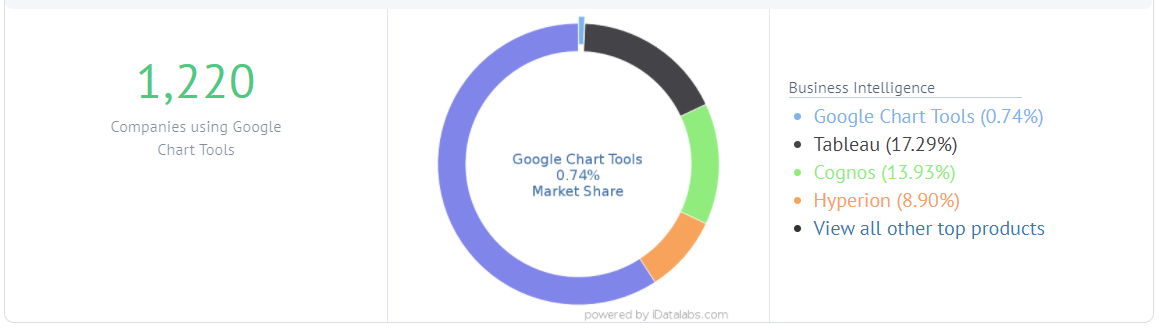
\includegraphics[width=1.0\columnwidth]{paper2/Figure 1.png}
  \caption{Comparision of companies using Google Chart Vs Tableau and Other Programs
  \cite{Idatalabs}}
  \label{fig:Figure 1} 
\end{figure}

As shown in Figure 1\ref{fig:Figure 1}, One can see that more companies use Tableau than Google Charts. Please note, the blue text that says click to view all other to products is a collection of other companies, which are not all displayed in the pie chart, because there are many other companies that do data visualization and analytics. Please visit this link https://idatalabs.com/tech/business-intelligence to see the rest of the rest of the companies. Google Chart and Tableau, and all those other products are good to use for data visualization, but we can even go a step further with programing languages such as Python and R. 

\section{Python}
“Python is an interpreted, object-oriented, high-level programming language with dynamic semantics.” Python is built for rapid application development, scripting, or glue language to link present components collectively. (Python Software Foundation, 2001-2017) This language is not however just limited to this. It can be used to make games, predictive models, make apps, work with other languages to build websites, investigate data to find collations, calculate averages and standard deviations, and build algorithms to solve complex problems such as in Artificial Intelligence. In addition, it has built in libraries that can allow the user to plot charts and create visuals from data. No wonder the Python Software Website says “Often, programmers fall in love with Python because of the increased productivity it provides” (Python Software Foundation, 2001-2017). Returning to the visual aspect, Python does not have many decorative visualizations as Tableau, but it offers of broader range of functionality, and a way to explore complex problems, and create solutions, which can be turned into visuals for people to better understand what’s happening. 
So how do visuals work in Python? Well according to an article called 9 Popular Ways to Perform Data Visualization in Python written by Sunil Ray from the Analytics Vidhya website, there are two libraries in Python called Matplotlib and Seaborn. Matplotib allows users to produce 2D and limited 3D graphic content. It also enables creation of animations as well. The other library is Seaborn, allows creation of informative and statistical graphs. Seaborn also provides many options such as “built in themes, color palettes, functions and tools to visualize univariate, bivariate, linear regression, matrices of data, statistical time series etc., which lets us to build complex visualizations.” (Sunil Ray, 2015)
In his article, Sunil Ray goes to show 9 examples of visualization he makes from the following Data set (Table 1):

\begin{figure}[htb]
  \centering
  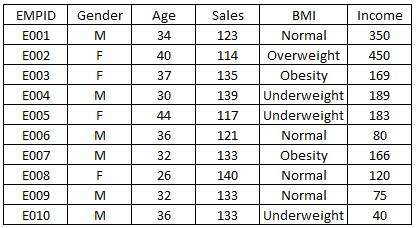
\includegraphics[width=1.0\columnwidth]{paper2/Table 1.png}
  \caption{Data Set Provided by Sunil Ray
  \cite{Sunil Ray }}
  \label{fig:Table 1} 
\end{figure}

From this data set, let’s look at three visualizations created by Sunil, to see more visit https://www.analyticsvidhya.com/blog/2015/05/data-visualization-python/.  

He starts off by importing the Matplotlib and Seaborn libraries into his Python text editor by using this call function, import matplotlib.pyplot as plt, this provides access to the chart capabilities in Matplotlib and Seaborn.
Then he imports the Pandas library as, import pandas as pd, “Pandas is a Python package providing fast, flexible, and expressive data structures designed to make working with relational or labeled data both easy and intuitive. It aims to be the fundamental high-level building block for doing practical, real world data analysis in Python.” (Pydata, 2017) 
Next he Imports his data frame, which is the date set above in the table along with pandas processing and reading that data set through the code, df=pd.read_excel("E:/First.xlsx", "Sheet1"

The three visulizations below are, a histogram showing age distribution (Graph 1), a box plot to show the spreading of ages based on the five elements: the min age, first quartile age, median age, third quartile age, and max age (Graph 2). He creates a violin plot (Graph 3) to show the relation between age and gender of the data set in the table above.

\begin{figure}[htb]
  \centering
  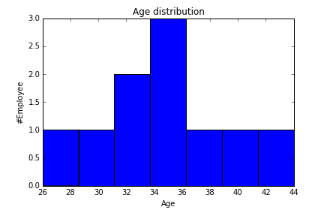
\includegraphics[width=1.0\columnwidth]{paper2/Graph 1.png}
  \caption{Age Distribution Histogram
  \cite{Sunil Ray }}
  \label{fig:Graph 1} 
\end{figure}

The python code for this histogram is:
fig=plt.figure() 
ax = fig.add_subplot(1,1,1)
ax.hist(df['Age'],bins = 7) 
plt.title('Age distribution')
plt.xlabel('Age')
plt.ylabel('#Employee')
plt.show()

\begin{figure}[htb]
  \centering
  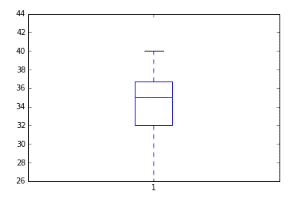
\includegraphics[width=1.0\columnwidth]{paper2/Graph 2.png}
  \caption{Age Spread Box Plot
  \cite{Sunil Ray }}
  \label{fig:Graph 2} 
\end{figure}

The python code for this Box plot is:
fig=plt.figure()
ax = fig.add_subplot(1,1,1)
#Variable
ax.boxplot(df['Age'])
plt.show()

\begin{figure}[htb]
  \centering
  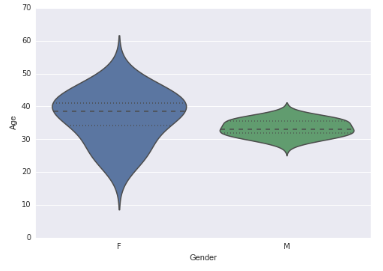
\includegraphics[width=1.0\columnwidth]{paper2/Graph 3.png}
  \caption{Age Comparision Between Genders Violin Plot
  \cite{Sunil Ray }}
  \label{fig:Graph 3} 
\end{figure}

The python code for this violin plot is:
sns.violinplot(df['Age'], df['Gender']) #Variable Plotsns.despine()

Note these are example of what Python can do, however someone can contend that the same results can be achieved in excel. Yes, this can be done in excel, but what happens if one has over hundreds of thousands of data from different sources. Excel can crush if there is too much information and depending on the capabilities of the computer. Therefore, Python can be a program to get around this. Another program like Python that will do visualizations is R. 

\section{R}
R is a programming language and a landscape for arithmetical computing and visuals. “R provides a wide variety of statistical (linear and nonlinear modelling, classical statistical tests, time-series analysis, classification, clustering, …) and graphical techniques, and is highly extensible.” (R Foundation) The R Foundation website goes on to say that R’s strength comes from the ease in which publication plots can be produced, in addition to the mathematical codes and workings that are available for use. Furthermore, reaching outside of the default settings for the graphics in R, the user retains control and can explore into options. This can be done by importing the package ggplot2 in R Studio, which will give you access to a wide range of graphics options like the ones found in Matplotlib and Seaborn through Python. According to the R Foundation, R has a built-in documentation format like Latex. (R Foundation) However, users still have an option to use Latex (specifically MiKTeX) with R. The Latex project says, Latex is a system that prepares documents for publication and communication for scientific documents, but it can be used for most publications. (Latex Project) Let look at how visuals can be produced using R and Latex. 

*Please note, the following example of R code with Latex is an example made by Jacob tibenkana and Jeremy Driscoll using the Titanic data pulled from Kaggle is a public online community of individuals (data analysts, data scientists, and others) that uses Pyrhon to investigate real world data examples, however here we will be looking at the data from an R perspective rather than through Python. To begin we need to download the following: R, R studio, and MikTeX (version of Latex). 
In R Studio, we set the file we are working with to Knitr, which allows to knit Python with Latex. Then we import the following packages, library(knitr), library(ggplot2), library(dplyr), library(tidyr). Think of these like the Python Libraries that were imported in Sunil’s examples above.
Library(knitr) allows for coupling of R with Latex, Library(ggplot2) allows for access to a wide range of graphics in R, Library(dplyr) and Library(tidyr) allows for exploration and processing of the Titanic data and organize it in tables so we can refer to ggplot2 for the graphics we want to display.
In R studio, the following will be displayed on line one:
\documentclass{article}, this is the beginning of the Latex shell and we can type the test we want here to describe the R Code that will follow. For a visual of how this looks in R Studio, please refer to the appendix below. 

Next the R code with Latex is displayed as:

%\begin{document}
<<echo=FALSE>>=
library(knitr)
library(ggplot2)
library(dplyr)
library(tidyr)
df<-read.csv("train.csv",stringsAsFactors = FALSE)
@
<<>>=
ggplot(data=df,aes(x=Sex))+geom_bar()
@
<<>>=
tb<-df%>%group_by(Sex,Survived)%>%summarise(Sum=n())
colnames(tb)<-c("Sex","Survived","Sum")
tb$Survived<-ifelse(tb$Survived==0,"No","Yes")
kable(tb)
@
<<>>=
ggplot(tb)+geom_col(aes(x=Sex,y=Sum,fill=Survived))
@
<<>>=
df$Agegroups<-ifelse(df$Age<10,"0-9",
              ifelse(df$Age<20,"10-19",
              ifelse(df$Age<30,"20-29",
              ifelse(df$Age<40,"30-39",
              ifelse(df$Age<50,"40-49",
              ifelse(df$Age<60,"50-59",
              ifelse(df$Age<70,"60-69",
              ifelse(df$Age<80,"70-79",NA))))))))
tb<-df%>%group_by(Agegroups,Survived)%>%summarise(Sum=n())%>%ungroup()
tb$Survived<-ifelse(tb$Survived==0,"No","Yes")
tb<-na.omit(tb)
x<-data.frame(Agegroups="70-79", Survived="Yes",Sum=0,stringsAsFactors = FALSE)
tb<-rbind(tb,x)
tb2<-tb%>%spread(Survived,Sum)
kable(tb2)
@
<<>>=
ggplot(tb)+geom_col(aes(x=Agegroups,y=Sum,fill=Survived),position="dodge")+xlab("Age Groups")
@
<<>>=
Ave<-df%>%group_by(Survived)%>%summarise("Mean Age"=mean(Age,na.rm = TRUE),"Mean of Siblings and Spouse"=mean(SibSp,na.rm = TRUE))
Ave$Survived<-ifelse(Ave$Survived==0,"No","Yes")
kable(Ave)
@:

%\end{document}

This code will produce the following visuals in a pdf report:

\begin{figure}[htb]
  \centering
  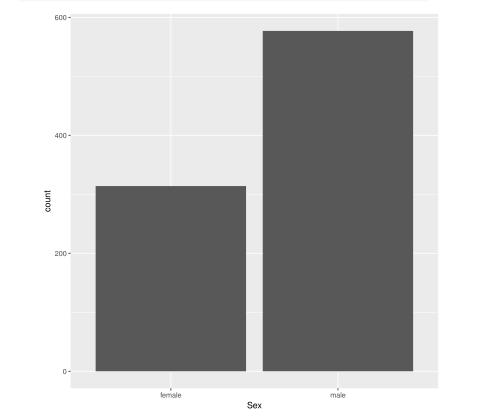
\includegraphics[width=1.0\columnwidth]{paper2/Graph 4.png}
  \caption{Bar Graph of Gender Representation on Titanic
  \cite{Tibenkana and Driscoll, Data Set from kaggle}}
  \label{fig:Graph 4} 
\end{figure}

This bar graph (Graph 4) shows how many women and men boarded the Titanic. As one can see there were more men than women that were on the Titanic based on the data set that was provided from Kaggle.

\begin{figure}[htb]
  \centering
  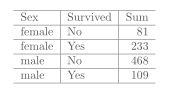
\includegraphics[width=1.0\columnwidth]{paper2/Table 2.png}
  \caption{Survived Vs Did Not Survive Per Gender Table
  \cite{Tibenkana and Driscoll, Data Set from Kaggle}}
  \label{fig:Table 2} 
\end{figure}

We can also call on certain information from the Data set and organize it to present it in a table (Table 2). For example, we can look at how many people survived vs did not survive per gender.

\begin{figure}[htb]
  \centering
  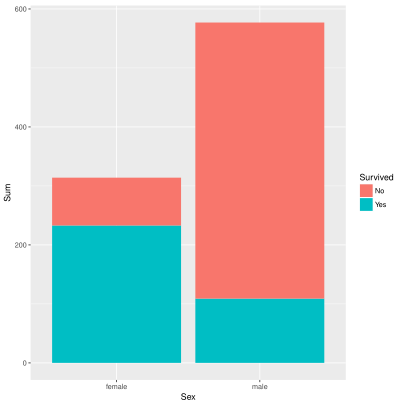
\includegraphics[width=1.0\columnwidth]{paper2/Graph 5.png}
  \caption{Stacked Bar Graph of Survived Vs Did Not Survive Per Gender
  \cite{Tibenkana and Driscoll, Data Set from Kaggle}}
  \label{fig:Graph 5} 
\end{figure}

The data in Table 2 above can be graphed as a stacked bar graph (Graph 5). As one can see, there were more men on board than women, but more women survived than men during the crash and sinking of the Titanic. The reason for why more women survived than men can also be another element to investigate using a statistical approach with R. However, to do this, we would need more data on this event than we have in the data set that was provided from kaggle. 

\begin{figure}[htb]
  \centering
  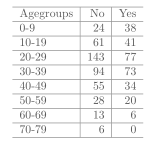
\includegraphics[width=1.0\columnwidth]{paper2/Table 3.png}
  \caption{Survived Vs Did Not Survive Per Age Group
  \cite{Tibenkana and Driscoll, Data Set from Kaggle}}
  \label{fig:Table 3} 
\end{figure}

Next, we can go a step further and look at the age ranges of the people who survived vs those that did not survive. This is shown in Table 3. Here we have age groups based on a nine-year span between the ages of 0 to 79. Column No represents the people who did not survive in that age group and column Yes represents, the individuals that survived within those age groups. This data can then be displayed in a side to side column graph (Graph 6) below, giving a visual of the people who survived vs who did not survive within their respected age groups.

\begin{figure}[htb]
  \centering
  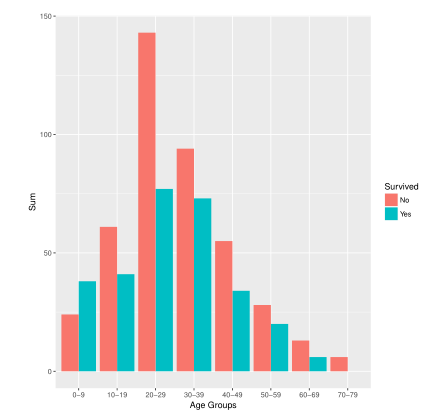
\includegraphics[width=1.0\columnwidth]{paper2/Graph 6.png}
  \caption{Sided by Side Column Chart of Survived Vs Did Not Survive Per Age Group
  \cite{Tibenkana and Driscoll, Data Set from Kaggle}}
  \label{fig:Graph 6} 
\end{figure}

From this graph we can see that the most people who survived were in their 20s and the most people who did not survive were also in their 20s as well. No one over the age of 70 survived. In terms of a survival ratio across all age groups, the 0 to 9 years old age group had more survivals than losses while age 20 to 29 had more loses than survivals.

In the code above, R is also calculating the average of survived vs not survived based on age. It turns out that the average age of people who survived was 30.6 and the average age of those who did not survive was 28.34. These are some of the easy computations and visuals that R can produce, however it can do even more complex statistical computations. 

\section{Conclusion} 
To conclude, we have moved from the industrial age and live in the informational age. We still rely on machinery from the industrial age, but the age of information is driving change and processes today. For example, machines today are using information (programming) to build other machines and to operate without the supervision of a people. However, there has to be a general understanding of the information or data before we can put it to use, and a manner in which people can understand this information is through visuals that can be brought about using the programs and products such as Python, R, tableau, etc.
 
\section{Appendix} 
 \begin{figure}[htb]
  \centering
  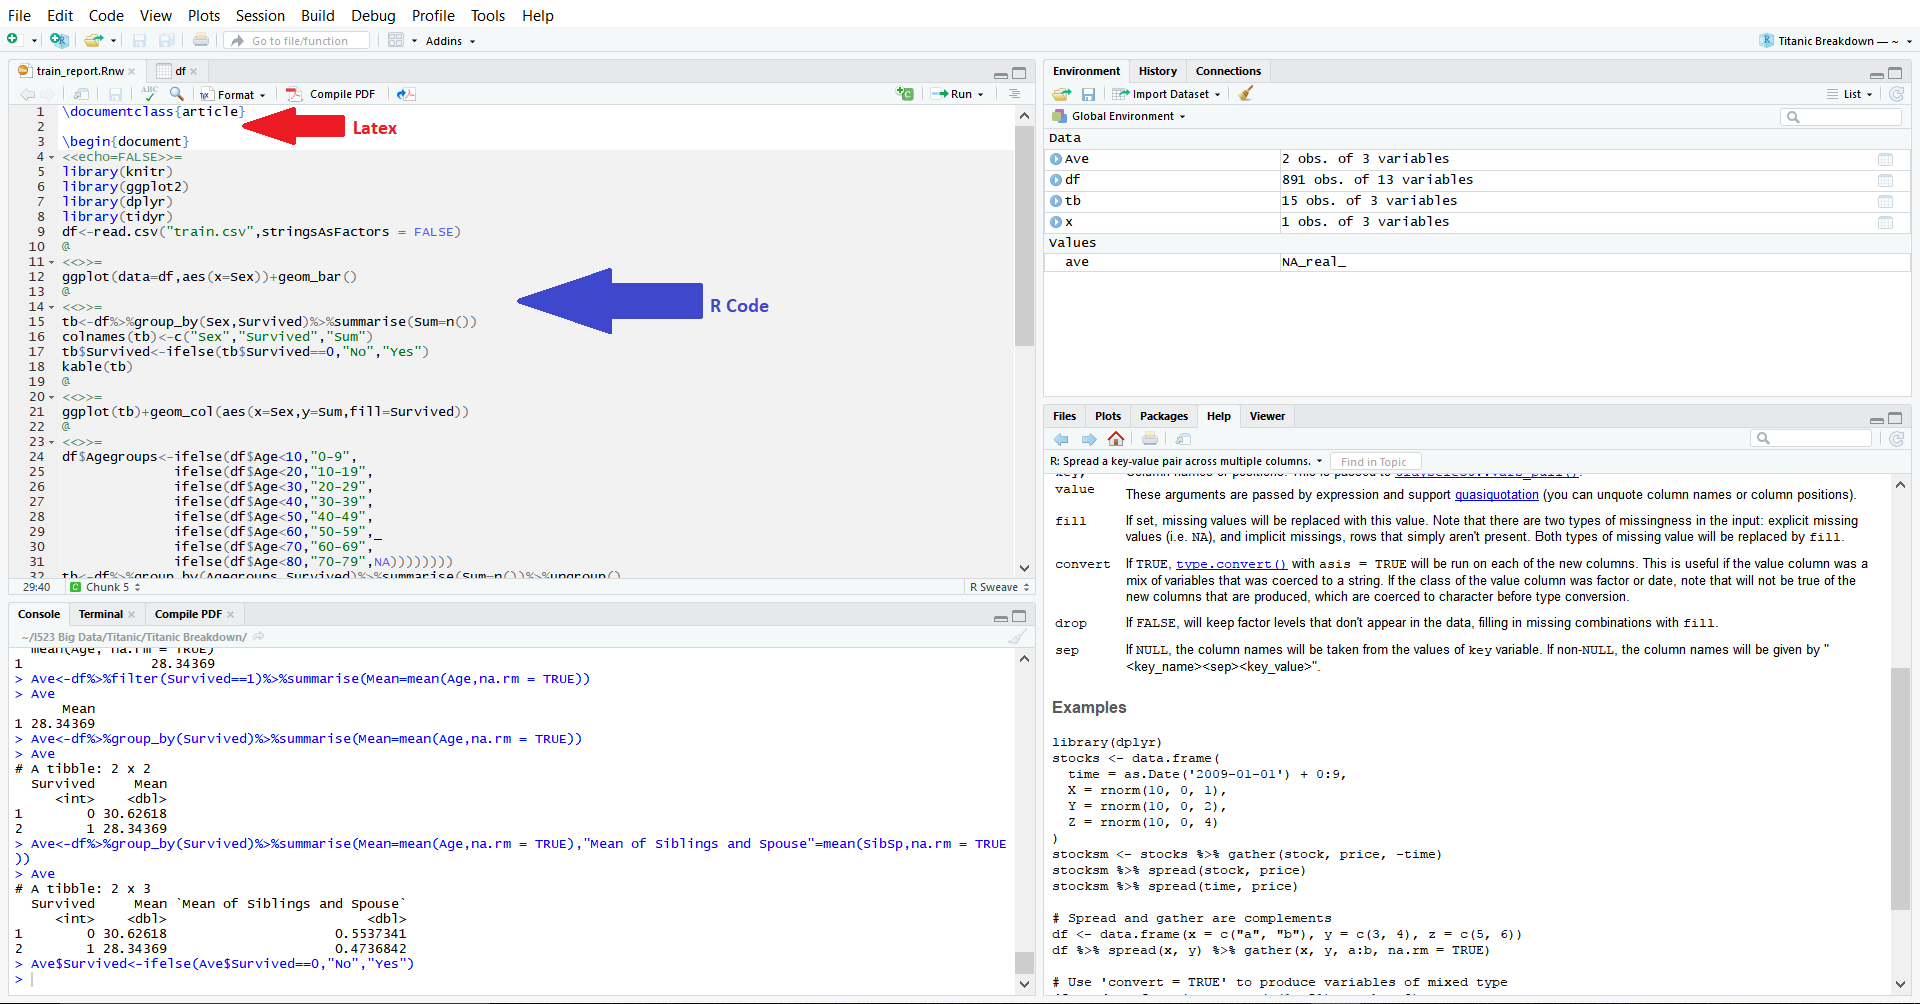
\includegraphics[width=1.0\columnwidth]{paper2/Latex With R Code in R Studio.png}
  \caption{Working in R Studio, Latex with R Code
  \cite{Tibenkana and Driscoll}}
  \label{fig:Latex With R Code in R Studio} 
\end{figure}
 
\begin{acks}

The authors would like to thank professor Gregor von Laszewski and his associates for providing the template code on which I wrote this paper.

\end{acks}

\bibliographystyle{ACM-Reference-Format}
\bibliography{report} 

\section{Bibtex Issues}
\todo[inline]{Warning--no journal in Bhatt10}
\todo[inline]{(There was 1 warning)}
\section{Issues}

\DONE{Example of done item: Once you fix an item, change TODO to DONE}

\subsection{Formatting}

    \TODO{Incorrect number of keywords or HID and i523 not included in the keywords}

\subsection{Writing Errors}

    \TODO{Spelling errors}
    \TODO{Do not use the phrase {\em In this paper/report we show} instead use {\em We show}. It is not important if this is a paper or a report and does not need to be mentioned}

\subsection{Citation Issues and Plagiarism}

    \TODO{Claims made without citations provided}
    \TODO{Need to paraphrase long quotations (whole sentences or longer)}

\subsection{Character Errors}

    \TODO{Erroneous use of quotation marks, i.e. use ``quotes'' , instead of " "}
    \TODO{If you see a figure and not a figure in text you copied from a text that has the fi combined as a single character}

\subsection{Structural Issues}

    \TODO{The paper has less than 2 pages of text, i.e. excluding images, tables and figures}


\end{document}

\section{Bibtex Issues}
\todo[inline]{Warning--no journal in Bhatt10}
\todo[inline]{(There was 1 warning)}
\section{Issues}

\DONE{Example of done item: Once you fix an item, change TODO to DONE}

\subsection{Formatting}

    \TODO{Incorrect number of keywords or HID and i523 not included in the keywords}

\subsection{Writing Errors}

    \TODO{Spelling errors}
    \TODO{Do not use the phrase {\em In this paper/report we show} instead use {\em We show}. It is not important if this is a paper or a report and does not need to be mentioned}

\subsection{Citation Issues and Plagiarism}

    \TODO{Claims made without citations provided}
    \TODO{Need to paraphrase long quotations (whole sentences or longer)}

\subsection{Character Errors}

    \TODO{Erroneous use of quotation marks, i.e. use ``quotes'' , instead of " "}
    \TODO{If you see a figure and not a figure in text you copied from a text that has the fi combined as a single character}

\subsection{Structural Issues}

    \TODO{The paper has less than 2 pages of text, i.e. excluding images, tables and figures}


\end{document}
